\documentclass{article}

% NeurIPS 2026 double-blind workshop format.
\PassOptionsToPackage{numbers,compress}{natbib}
\usepackage[dblblindworkshop]{neurips_2026}
\workshoptitle{Verify-Agents Workshop}

% ========== Core packages ==========
\usepackage[utf8]{inputenc}
\usepackage[T1]{fontenc}
\usepackage{amsmath,amssymb,mathtools}
\usepackage{booktabs}
\usepackage{array}
\usepackage{multirow}
\usepackage{graphicx}
\usepackage{hyperref}
\usepackage{url}
\usepackage{xcolor}
\usepackage{microtype}
\usepackage{enumitem}
\usepackage{placeins}
\usepackage{tikz}
\usetikzlibrary{arrows.meta,positioning,calc}

\hypersetup{
  colorlinks=true, linkcolor=blue, citecolor=blue, urlcolor=blue,
  pdftitle={When Gold Trajectories Become Unreachable},
  pdfauthor={Anonymous}
}

\title{Invocation-Level Reliability of Tool-Using Agents }
\author{
  Anonymous Author(s) \\
  Affiliation \\
  Address \\
  \texttt{email@domain}
}
\date{}

\begin{document}
\maketitle

% =====================================================================
\begin{abstract}
An early tool-call error can corrupt every downstream input even when an agent subsequently applies the right local rule. We isolate this effect with matched evaluations under a correct baseline history and the model's own free-running history. For tasks of depth $d$, their pooled invocation rates $\bar p_d$ and $\bar g_d$ define a fit-free relative propagation loss $L_d=1-\bar g_d/\bar p_d$. Across five open-weight models on controlled routing tasks, the two 7--8B models lose about 68\% of baseline capability by depth 6; stronger models mostly remain at ceiling. Our main result is a construct-validity condition for trajectory scoring. Let $Y_k^*$ be the canonical next target after a divergence and $H_k$ the agent-observable history. If $Y_k^*$ has conditional guessing probability at most $\epsilon_k$ given $H_k$, then any fixed-gold scorer credits the agent with probability at most $\epsilon_k$, regardless of its local competence. Gold-agreement severity is therefore driven to a scorer-imposed boundary, and observed reconvergence cannot measure behavioral recovery. \textbf{Fixed reference alone is not sufficient}: the result applies when the canonical target becomes unreachable or unpredictable, and excludes reconstructible targets and evaluators that accept alternative states or milestone paths. Our hidden-constant tasks instantiate the condition: 0 of 869 corrupted-context calls match gold, and 0 of 580 opportunities reconverge. Conditional-on-state replay instead asks whether a call correctly continues from the state the agent actually holds; it yields interior severity estimates of 0.149 and 0.316 and requires no new model queries. Alternative absolute-gap and error-amplification summaries give the same qualitative depth trend.
\end{abstract}

% =====================================================================
\section{Introduction}

Language model agents interact with external systems by emitting structured \emph{tool calls}: each call names a function (e.g.\ \texttt{get\_weather}, \texttt{query\_database}) and fills its required arguments. A call can fail by selecting the wrong function (\emph{selection error}) or by providing incorrect argument values (\emph{argument error}). In a multi-step task where each call's output feeds into the next, a single wrong call early in the chain corrupts the inputs to every downstream call, even if the model reasons correctly from that point on.

Many benchmarks report task success or agreement with a canonical call, without separately measuring selection, arguments, and the downstream effect of an earlier error. State-based benchmarks allow alternative solutions, and process benchmarks annotate individual steps, but neither directly supplies the matched baseline/free-running contrast studied here. These distinctions matter because local incompetence, state corruption, and ordinary later-step difficulty require different interventions.

We introduce a protocol that makes this distinction. A call is \emph{correct} when it selects the appropriate tool and supplies the arguments required by the scoring regime. We measure it under two matched conditions: a \emph{baseline} condition with a guaranteed-correct history and a \emph{free-running} condition with the model's own prior outputs. Their gap measures the loss associated with accumulated state corruption while controlling for the prompts and later-step difficulty present in the baseline arm.

The study began as an empirical comparison and exposed a construct-validity problem. When divergence makes the canonical next target unpredictable from everything the agent observes, gold agreement measures target reachability rather than the competence of the next call. This is not a property of every fixed-reference benchmark: it depends on an explicit unreachable-target condition. We state that condition, give a counterexample, and separate the resulting scorer-imposed boundary from the model's behavior.

\paragraph{Contributions.}
\begin{enumerate}[leftmargin=*,itemsep=1pt,topsep=1pt,parsep=0pt]
  \item A disaggregated measurement protocol that separately scores tool selection and argument correctness under matched baseline and free-running conditions, with a routing-task design where selection errors, not just argument errors, propagate.
  \item A formal unreachable-target condition under which canonical gold agreement is bounded by the target's conditional guessing probability, making gold-based severity and reconvergence scorer-dominated rather than behavioral.
  \item A remedy, conditional-on-state scoring, where each call is judged against what would be correct given the value the model actually holds: implemented and applied retrospectively to cached completions at zero marginal cost.
  \item Robustness summaries beyond $L_d$ (absolute excess error and error amplification), plus per-model diagnostics for rule discrimination and error position.
\end{enumerate}

% =====================================================================
\section{Related Work}

Toolformer~\cite{schick2023toolformer}, ReAct~\cite{yao2023react}, and Gorilla~\cite{patil2023gorilla} established tool-augmented agents. ToolLLM~\cite{qin2024toolllm}, StableToolBench~\cite{guo2024stabletoolbench}, API-Bank~\cite{li2023apibank}, and BFCL~\cite{patil2025bfcl} emphasize task success or agreement with reference calls. RoTBench~\cite{ye2024rotbench} and MTU-Bench~\cite{wang2025mtubench} separate selection from argument accuracy; FuncBenchGen~\cite{maekawa2025funcbenchgen} generates fresh dependency-graph tasks and reports stale-value failures. Our distinct estimand is the matched change in invocation correctness when gold history is replaced by the same model's history.

Not all agent evaluation uses one canonical trajectory. $\tau$-bench~\cite{yao2024taubench} grades final environment state; AppWorld~\cite{trivedi2024appworld} uses state-based unit tests that permit multiple solutions; ToolSandbox~\cite{lu2024toolsandbox} evaluates intermediate and final milestone DAGs over arbitrary trajectories. These methods avoid the unreachable-canonical-target failure but primarily measure outcome or milestone completion, not local post-divergence competence. Section~\ref{sec:central-result} states the narrower condition under which canonical-call scoring becomes scorer-dominated.

Process-oriented work is complementary. AgentProcessBench~\cite{fan2026agentprocessbench} provides human step labels and an explicit propagation rule, while FALAT~\cite{rafi2026falat} traces dependencies to separate decisive errors from inherited downstream failures. Relign~\cite{xu2025relign}, Hammer~\cite{lin2024hammer}, and representation-level detection~\cite{healy2026internal} instead reduce or detect the production of an incorrect call. We intervene on history to quantify propagation and compare gold-agreement with conditional-on-state scoring.

% =====================================================================
\section{Method}

\begin{figure}[ht]
\centering
\resizebox{0.98\textwidth}{!}{%
% Methodology diagram: two-arm protocol + three-state propagation model
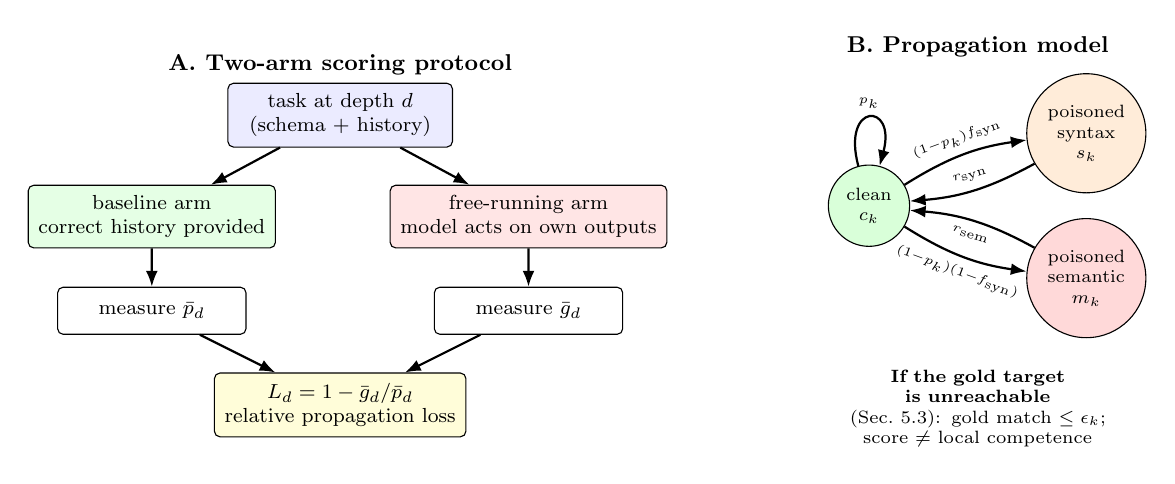
\begin{tikzpicture}[
    box/.style={draw, rounded corners=2pt, minimum height=0.65cm, align=center, font=\footnotesize, inner sep=4pt},
    state/.style={draw, circle, minimum size=0.9cm, font=\scriptsize, align=center},
    arrow/.style={-{Latex[length=2mm]}, thick},
    dashedarrow/.style={-{Latex[length=2mm]}, dashed},
    scale=0.92, every node/.style={transform shape}
]

% --- Panel A: two-arm protocol ---
\node[box, fill=blue!8, minimum width=3.1cm] (task) at (0,3.4) {task at depth $d$\\(schema + history)};
\node[box, fill=green!10, minimum width=3.4cm] (tf) at (-2.6,2.0) {baseline arm\\correct history provided};
\node[box, fill=red!10, minimum width=3.4cm] (free) at (2.6,2.0) {free-running arm\\model acts on own outputs};
\node[box, minimum width=2.6cm] (pt) at (-2.6,0.7) {measure $\bar p_d$};
\node[box, minimum width=2.6cm] (gt) at (2.6,0.7) {measure $\bar g_d$};
\node[box, fill=yellow!15, minimum width=3.4cm] (Lt) at (0,-0.6) {$L_d = 1 - \bar g_d/\bar p_d$\\relative propagation loss};

\draw[arrow] (task) -- (tf);
\draw[arrow] (task) -- (free);
\draw[arrow] (tf) -- (pt);
\draw[arrow] (free) -- (gt);
\draw[arrow] (pt) -- (Lt);
\draw[arrow] (gt) -- (Lt);

% --- Panel B: three-state Markov model, to the right ---
\begin{scope}[yshift=-0.45cm]
\node[state, fill=green!15] (C) at (7.3,2.6) {clean\\$c_k$};
\node[state, fill=orange!15] (S) at (10.3,3.6) {poisoned\\syntax\\$s_k$};
\node[state, fill=red!15] (M) at (10.3,1.6) {poisoned\\semantic\\$m_k$};

\draw[arrow] (C) to[bend left=12] node[above,font=\tiny,sloped]{$(1{-}p_k)f_{\mathrm{syn}}$} (S);
\draw[arrow] (C) to[bend right=12] node[below,font=\tiny,sloped]{$(1{-}p_k)(1{-}f_{\mathrm{syn}})$} (M);
\draw[arrow] (S) to[bend left=12] node[above,font=\tiny,sloped]{$r_{\mathrm{syn}}$} (C);
\draw[arrow] (M) to[bend right=12] node[below,font=\tiny,sloped]{$r_{\mathrm{sem}}$} (C);
\draw[arrow] (C) to[loop above] node[above,font=\tiny]{$p_k$} (C);

\node[font=\scriptsize, align=center, text width=3.5cm] at (8.8,-0.2) {\textbf{If the gold target is unreachable}\\(Sec.~5.3): gold match $\leq\epsilon_k$;\\score $\neq$ local competence};
\end{scope}

\node[font=\bfseries\small] at (0,4.1) {A.\ Two-arm scoring protocol};
\node[font=\bfseries\small] at (8.8,4.35) {B.\ Propagation model};

\end{tikzpicture}%
}
\caption{(A) Matched evaluation at task depth $d$: pooled baseline and free-running invocation rates define $L_d$. (B) A separate step-indexed propagation model. Under the unreachable-target condition of Section~\ref{sec:central-result}, canonical gold agreement is bounded by target predictability rather than local competence.}
\label{fig:methodology}
\end{figure}

\subsection{Definitions}
\label{sec:definitions}

A task of dependency depth $d$ contains calls indexed by position $k\in\{1,\ldots,d\}$. For task $i$, let $B_{i,k}$ and $F_{i,k}$ indicate invocation correctness in the baseline and free-running arms. With $N_d$ tasks at depth $d$, the reported depth-level estimands are
\begin{equation}
\bar p_d=\frac{1}{N_dd}\sum_{i=1}^{N_d}\sum_{k=1}^{d}B_{i,k},\qquad
\bar g_d=\frac{1}{N_dd}\sum_{i=1}^{N_d}\sum_{k=1}^{d}F_{i,k}.
\end{equation}

\begin{itemize}[leftmargin=*,itemsep=1pt,topsep=1pt,parsep=0pt]
  \item \textbf{Pooled baseline correctness $\bar p_d$}: invocation accuracy with a guaranteed-correct prior history.
  \item \textbf{Pooled free-running correctness $\bar g_d$}: invocation accuracy with the model's own prior outputs.
  \item \textbf{Relative propagation loss} $L_d \coloneqq 1-\bar g_d/\bar p_d$. We also report the absolute gap $A_d=\bar p_d-\bar g_d$ and error amplification $E_d=(1-\bar g_d)/(1-\bar p_d)$.
\end{itemize}

$L_d$ is descriptive and invocation-pooled; it is not the stepwise quantity in the Markov recurrence below. Calls from one task are dependent, so inferential intervals must resample matched tasks jointly rather than treat $N_dd$ calls as independent. The conclusions emphasized here are the paired point-estimate pattern, the directly observed corrupted-context counts, and the scorer theorem.

\subsection{A propagation model with recovery}
\label{sec:propagation-model}

For interpretation only, we model step-indexed context as clean, poisoned-by-syntax, or poisoned-by-semantics (Figure~\ref{fig:methodology}B). Let $p_k$ be correctness at position $k$ under clean history and $f_{\mathrm{syn}}(k)$ the syntactic share of new errors. With origin-specific recovery rates $r_{\mathrm{syn}},r_{\mathrm{sem}}$ and poisoned-state correctness $\rho_k=(1-\pi)p_k$, occupancies evolve as
\begin{align}
c_{k+1} &= c_kp_k+s_kr_{\mathrm{syn}}+m_kr_{\mathrm{sem}}, \quad
s_{k+1} = c_k(1-p_k)f_{\mathrm{syn}}(k)+s_k(1-r_{\mathrm{syn}}), \\
m_{k+1} &= c_k(1-p_k)(1-f_{\mathrm{syn}}(k))+m_k(1-r_{\mathrm{sem}}).
\end{align}
The model-implied step accuracy is $g_k^{\mathrm{model}}=c_kp_k+(s_k+m_k)\rho_k=p_k(1-\pi x_k)$ for poisoned mass $x_k=s_k+m_k$. We fit $\pi,r_{\mathrm{syn}},r_{\mathrm{sem}}$ hierarchically (PyMC, NUTS) as a cautionary diagnostic, not as the estimator of $L_d$. Section~\ref{sec:central-result} explains why gold-agreement data do not identify the intended behavioral interpretation of these parameters under an unreachable target.

\subsection{Task design}

Each task is a hidden dependency graph over deterministic executable functions, giving exact ground truth per call and direct control of depth ($\{1,2,4,6,8\}$). Tool outputs lie in a size-$M$ space ($M=100{,}000$) and take the form $(a\cdot\mathrm{arg}+b)\bmod M$, with per-tool constants omitted from the schema. Section~\ref{sec:central-result} does not infer unpredictability from secrecy alone; it states the conditional target-predictability assumption required for the bound.

\textbf{Routing tasks (primary)}: the correct next tool is a parity rule applied to the incoming value, not a pre-announced order, so a wrong choice changes what is correct downstream. Selection is scored \emph{conditionally}, against the tool correct given the value the model actually holds, with divergence from gold recorded separately, so applying the rule correctly to a corrupted input is not misclassified as selection failure. \textbf{Linear tasks (control)}: order announced, argument copied verbatim. Pilot runs were degenerate ($\bar p_d=\bar g_d=1.000$ on two models), and the full null arm was not executed (Section~\ref{sec:limitations}).

\subsection{Protocol and suite}

We score selection against the tool appropriate for the value in the model's actual state and, for the primary gold-agreement analysis, score arguments against the canonical trajectory. Digit-only JSON strings are coerced to integers, so formatting is not a value error. Errors are syntactic (parse/schema failure) or semantic (executes but is wrong). Both arms use the same within-step retry budget. Conditional-on-state replay replaces the argument target with the argument implied by the model's actual state, making the selection and argument criteria symmetric.

We evaluated five open-weight models available through one hosted API: \texttt{llama-3.1-8b-instant}, \texttt{allam-2-7b}, \texttt{qwen3.6-27b}, \texttt{gpt-oss-120b}, and \texttt{llama-3.3-70b-versatile}. Greedy decoding, fixed seeds, and caching by (model, calling mode, exact prompt) make each benchmark prompt deterministic. Provider constraints produced unequal nested sample sizes and prevented balanced family, proprietary-model, and calling-mode comparisons; we draw no claims along those axes.

Models run \textbf{nested prefixes} of one task suite, sized per model to its own measured token allowance. Task identity depends only on $(\mathrm{depth},k,\mathrm{seed})$, never on how many tasks were requested, so cross-model contrasts on the shared prefix remain exactly paired while each model's own estimate uses its full $n$.

% =====================================================================
\section{Data Collected}
\label{sec:data}

All figures come from a dataset frozen at 14:09 on 2026-08-17; no missing model--depth cell is extrapolated.

\begin{table}[h]
\centering
\caption{Per-model sample sizes at the freeze.}
\label{tab:samples}
\footnotesize
\begin{tabular}{@{}lrrrrrrl@{}}
\toprule
Model & tasks & $d_1$ & $d_2$ & $d_4$ & $d_6$ & $d_8$ & status \\
\midrule
\texttt{llama-3.1-8b-instant} & \textbf{273} & 60 & 60 & 65 & 65 & 23 & only model at depth 8 \\
\texttt{allam-2-7b} & \textbf{225} & 60 & 60 & 65 & 40 & -- & usable \\
\texttt{gpt-oss-120b} & \textbf{108} & 26 & 26 & 28 & 28 & -- & usable \\
\texttt{qwen3.6-27b} & \textbf{98} & 26 & 26 & 28 & 18 & -- & usable \\
\texttt{llama-3.3-70b-versatile} & \textbf{49} & 12 & 12 & 13 & 12 & -- & usable, thin \\
\texttt{gpt-oss-20b} & \textbf{0} & -- & -- & -- & -- & -- & \textbf{excluded} \\
\bottomrule
\end{tabular}
\end{table}

\texttt{gpt-oss-20b} completed zero tasks after pilot calls consumed its daily allowance and is excluded from every empirical claim. Provider constraints explain the unequal sample sizes but are not treated as scientific findings.

% =====================================================================
\section{Results}
\label{sec:results}

\subsection{Propagation grows through depth 6 and exceeds baseline decay}
\label{sec:propagation-large}

\begin{figure}[t]
\centering
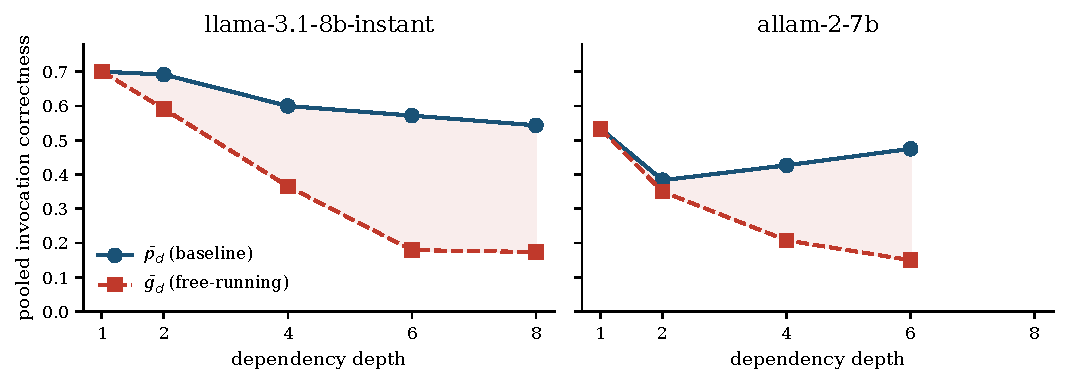
\includegraphics[width=0.98\textwidth]{fig_propagation_gap.pdf}
\caption{Pooled baseline correctness $\bar p_d$ versus pooled free-running correctness $\bar g_d$. The absolute gap widens through depth 6 and then plateaus for \texttt{llama-3.1-8b}; depth 1 is identical by construction.}
\label{fig:propagation-gap}
\end{figure}

Figure~\ref{fig:propagation-gap} and Table~\ref{tab:depth-results} show the core measurement. On \texttt{llama-3.1-8b}, $\bar p_d$ declines from 0.700 to 0.543 (22\% relative), while $\bar g_d$ declines to 0.174 (75\%). $L_d$ rises sharply through depth 6 and is essentially unchanged at depth 8 (0.686 vs.\ 0.680); we therefore claim growth followed by a plateau, not strict monotonicity or significant adjacent-depth differences.

\begin{table}[h]
\centering
\caption{Invocation-pooled depth estimands for the two high-$n$ models. Intervals are the reported 89\% intervals from the frozen paired analysis.}
\label{tab:depth-results}
\footnotesize
\begin{tabular}{@{}lrrrl@{}}
\toprule
\multicolumn{5}{c}{\texttt{llama-3.1-8b-instant}} \\
\midrule
depth $d$ & $\bar p_d$ & $\bar g_d$ & $L_d$ [89\% interval] & calls \\
\midrule
1 & 0.700 & 0.700 & \textbf{0.000} $[0.000,0.000]$ & 60 \\
2 & 0.692 & 0.592 & 0.145 $[0.082,0.222]$ & 120 \\
4 & 0.600 & 0.365 & 0.391 $[0.311,0.474]$ & 260 \\
6 & 0.572 & 0.179 & \textbf{0.686} $[0.607,0.766]$ & 390 \\
8 & 0.543 & 0.174 & \textbf{0.680} $[0.574,0.772]$ & 184 \\
\midrule
\multicolumn{5}{c}{\texttt{allam-2-7b}} \\
\midrule
1 & 0.533 & 0.533 & \textbf{0.000} $[0.000,0.000]$ & 60 \\
2 & 0.383 & 0.350 & 0.087 $[0.022,0.163]$ & 120 \\
4 & 0.427 & 0.208 & 0.514 $[0.429,0.600]$ & 260 \\
6 & 0.475 & 0.150 & \textbf{0.684} $[0.624,0.745]$ & 240 \\
\bottomrule
\end{tabular}
\end{table}

\textbf{$L_1=0$ exactly on every model}: both arms build an identical depth-1 prompt and share one cached response, providing an implementation invariant. At depth 6, \texttt{llama-3.1-8b} has identical baseline/free error counts at the first position (21/21), after which free-running errors rise while baseline errors remain approximately flat. The absolute gap and error-amplification summaries show the same through-depth-6 increase without dividing by baseline accuracy.

The lag association $\Delta_1=P(k{+}1\text{ correct}\mid k\text{ correct})-P(k{+}1\text{ correct}\mid k\text{ wrong})$ is positive for every model with errors ($+0.32$ to $+1.00$). It is descriptive rather than causal; its second term is zero under canonical gold agreement because of the unreachable-target mechanism below.

\subsection{Ceiling models, and where in a chain a model errs}
\label{sec:ceiling}

\begin{figure}[t]
\centering
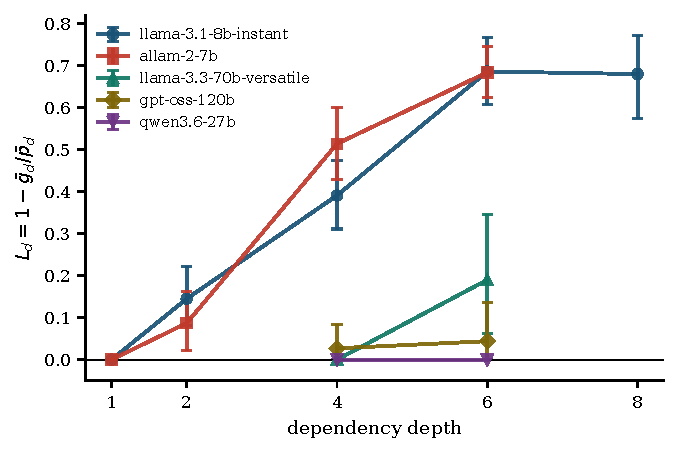
\includegraphics[width=0.62\textwidth]{fig_Lt_all_models.pdf}
\caption{$L_d$ versus depth for all usable models (89\% intervals). Three models remain near ceiling; \texttt{llama-3.3-70b-versatile} shows a positive depth-6 estimate.}
\label{fig:lt-all}
\end{figure}

Three models sit at or near ceiling ($\bar p_d=0.865$--$1.000$; Figure~\ref{fig:lt-all}), so $L_d\approx0$ is primarily a statement about task difficulty. On \texttt{llama-3.3-70b-versatile} at depth 4, 6 of 7 errors occur at a terminal position, leaving no downstream opportunity. At depth 6 its estimate is $L_6=0.190$ $[0.062,0.345]$, but the sample is thin. \texttt{gpt-oss-120b} has one fresh error, and \texttt{qwen3.6-27b} has zero errors across 298 free-running calls; neither supports a robustness claim.

An error at the terminal position cannot propagate, so a fixed-depth aggregate mixes error frequency with the remaining opportunity for downstream damage; $L_1=0$ is the limiting case. For \texttt{llama-3.1-8b}, terminal-error shares are 0.714 at $d=2$ and 0.197 at $d=6$, versus uniform-position baselines of 0.500 and 0.167. For \texttt{llama-3.3-70b-versatile}, the 6/7 terminal share at $d=4$ is suggestive but extremely uncertain. Terminal-error share should therefore accompany $L_d$, and cross-model comparisons require comparable position distributions.

\FloatBarrier

\subsection{When canonical gold agreement ceases to measure behavior}
\label{sec:central-result}

Let $H_k$ denote everything available to the agent before a post-divergence call, and let $Y_k^*$ be the canonical gold target used by the scorer. Define its conditional guessing probability
\begin{equation}
\epsilon_k(H_k)=\max_y P(Y_k^*=y\mid H_k).
\end{equation}

\paragraph{Proposition (unreachable-target bound).}
For any possibly randomized agent whose prediction $\widehat Y_k$ depends only on $H_k$,
\begin{equation}
P(\widehat Y_k=Y_k^*\mid H_k)\le \epsilon_k(H_k).
\end{equation}
Consequently, if $q_k^{\mathrm{gold}}$ is correctness in corrupted context and $p_k>0$ is clean-context correctness, gold-defined severity satisfies $\pi_k^{\mathrm{gold}}=1-q_k^{\mathrm{gold}}/p_k\ge1-\mathbb E[\epsilon_k]/p_k$. Across recovery opportunities $\mathcal K$, the probability of any chance reconvergence is at most $\sum_{k\in\mathcal K}\mathbb E[\epsilon_k]$.

\emph{Proof.} Conditional on $H_k$, sum over candidate outputs: $P(\widehat Y_k=Y_k^*\mid H_k)=\sum_yP(\widehat Y_k=y\mid H_k)P(Y_k^*=y\mid H_k)\le\max_yP(Y_k^*=y\mid H_k)$. The recovery statement is the union bound. \hfill$\square$

The proposition is about \emph{construct validity}: when $\epsilon_k$ is negligible, gold agreement cannot distinguish a locally competent continuation from arbitrary behavior. It does not say the operational statistic is numerically unidentified; rather, the statistic is pinned near a boundary that no longer represents the intended behavioral severity.

\paragraph{Instantiation in this suite.}
After divergence, canonical arguments depend on the hidden-constant output associated with the gold state. Under the generator assumption that this target is conditionally uniform over $M=100{,}000$ values, $\epsilon_k=10^{-5}$. We observe 0 gold matches among 869 corrupted-context calls and 0 canonical reconvergences among 580 opportunities. Even a pure-guess process has expected reconvergences $580/M=0.0058$, with probability of any such event at most 0.0058. Zero therefore carries essentially no information about whether the agent can apply the local routing/copy rule in its actual state.

If one nevertheless substitutes the scorer-implied boundary $\pi=1$ and zero canonical recovery into the step model, it collapses to $g_k^{\mathrm{model}}=c_kp_k$ and $c_k=\prod_{j<k}p_j$. A hierarchical fit to pooled aggregates returned severity posteriors of 0.92 and 0.73 despite zero observed post-divergence gold matches; $\hat R\le1.0005$, ESS $\ge5{,}823$, and zero divergences show only that the misspecified posterior was explored successfully: a targeted posterior predictive check finds 0 of 6{,}000 replicates reproducing the observed zero canonical matches among corrupted-context calls, against a predicted mean of 67.7.

\paragraph{Counterexample and scope.}
Fixed reference is not sufficient for the proposition. If $Y_k^*$ is reconstructible from the observable history, independent of the corrupted value, or reachable through reset/re-query actions, $\epsilon_k$ may be large and canonical recovery can be meaningful. Final-state unit tests and milestone-DAG evaluators can also accept alternative valid trajectories. Our claim is therefore restricted to canonical scoring under an empirically or structurally small $\epsilon_k$; it is not a blanket claim about execution match, AST match, or fixed references.

\subsection{A remedy: conditional-on-state scoring}
\label{sec:remedy}

Credit a call when it \emph{correctly continues from the value the model actually holds}, not when it matches the canonical state. Routing selection was already computed conditionally; replay adds the argument-side counterpart. Because every raw completion was cached, this required 881 cache reads and no new model queries.

\begin{figure}[ht]
\centering
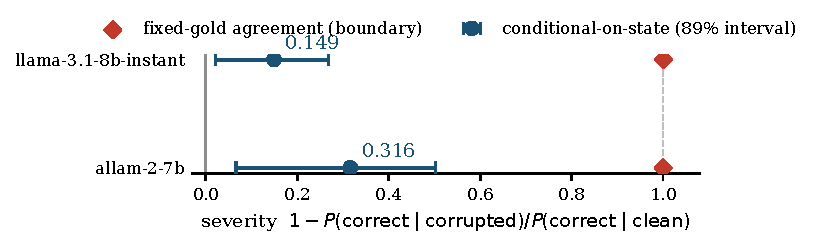
\includegraphics[width=0.78\textwidth]{fig_severity_comparison.pdf}
\caption{Gold-agreement severity is pinned at its boundary, whereas conditional-on-state replay yields interior estimates (reported 89\% intervals). The contrast is a change of estimand, not an improved fit to the same target.}
\label{fig:conditional-severity}
\end{figure}

Clean-context calls score identically under both rules (0.658 vs.\ 0.658), an implementation invariant. Conditional severity is 0.149 $[0.021,0.268]$ for \texttt{llama-3.1-8b} and 0.316 $[0.066,0.503]$ for \texttt{allam-2-7b}. Thus state corruption is associated with genuine loss of local rule application, but far less than the boundary value assigned by canonical gold agreement. Evidence is limited to two models and a weak copy-argument competence test.

\textbf{Trade-off.} Conditional scoring requires an executable transition model for the agent's actual state and does not imply end-task success. Canonical gold, conditional-on-state, milestone, and final-state scores answer different questions; none should be presented as a universal replacement.

\subsection{Rule-following is measurable directly, and aggregates hide it}
\label{sec:discrimination}

\begin{figure}[ht]
\centering
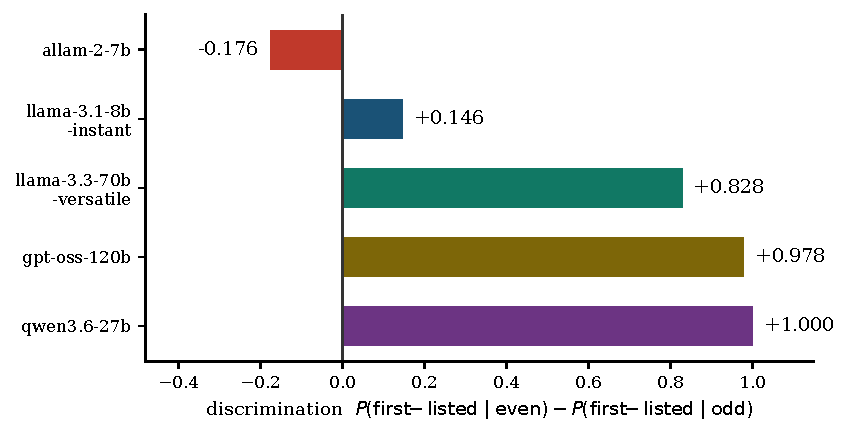
\includegraphics[width=0.62\textwidth]{fig_discrimination.pdf}
\caption{Discrimination, defined as $P(\text{first-listed}\mid\text{even})-P(\text{first-listed}\mid\text{odd})$, per model. Order matches the independently established reliability order of Section~\ref{sec:propagation-large}.}
\label{fig:discrimination}
\end{figure}

Define \textbf{discrimination} as $P(\text{first-listed}\mid\text{ref even})-P(\text{first-listed}\mid\text{ref odd})$: 0 means the rule is ignored, $+1$ perfect application, negative means \emph{anti}-correlated. Overall first-listed rates (0.478--0.497, four of five models) are indistinguishable and consistent with no position bias whatever; the \emph{same data}, conditioned on parity, resolves discrimination across the full range (Figure~\ref{fig:discrimination}), and the order matches reliability established independently in Section~\ref{sec:propagation-large}. \textbf{Discrimination is a per-model diagnostic of whether a model performs the task at all, invisible to any metric aggregated over the conditioning variable.}

Three qualitatively different relationships, not one spectrum: \texttt{qwen3.6-27b} \emph{derives} the rule ($+1.000$, zero errors in 298 steps, explicit reasoning trace); \texttt{llama-3.1-8b} \emph{weakly follows} it ($+0.146$, $z{=}4.7$); \texttt{allam-2-7b} is \emph{anti-correlated} ($-0.176$, $z{=}-5.0$): it picks the first-listed tool \emph{more} on odd refs (0.774) than even (0.597), where its accuracy is worst (0.223 vs.\ 0.595). \texttt{allam-2-7b}'s propagation loss is therefore not ``a weak model that errs more'' but a model \emph{not performing the routing task}.

\subsection{Two negative results}

\textbf{Untestable, not underpowered:} a hypothesised error-composition shift along the chain cannot be tested here because \textbf{389 of 389} clean-context errors are selection errors: on a copy-argument task there are only two ways to fail cleanly, mis-apply the parity rule (hard) or mis-transcribe a verbatim number (models never do). \textbf{Unresolved by design}: the suite offers two 2-point scale contrasts rather than 3--4, not comparable in kind (\texttt{llama} 8B$\to$70B dense, $8.75\times$; \texttt{gpt-oss} 20B$\to$120B, $6\times$ total but $\approx1.4\times$ active params). We report both axes and draw no scale conclusion, since the larger models sit at ceiling on these tasks.

% =====================================================================
\section{Pipeline Validation, and What Simulation Cannot Establish}
\label{sec:validation}

Before spending API budget we validated the full pipeline against six simulated policies with known ground truth, eliminating seven harness artifacts (retry-budget asymmetry, selection errors mis-attributed under poisoning, a contaminated syntactic-share estimator, among others). Two further artifacts were not coding errors, which is what makes them instructive: comparing carried value against \emph{expected argument} rather than \emph{previous gold output} is correct on a copy-argument task and silently wrong under any transform; and the simulated policies recovered by reading ground truth directly, out of band, through a channel no real model has. Correct code, correct configuration, invalid measurement. The second artifact is why the recovery channel was never estimable from observable data in any version of this pipeline.

Three principles follow, nested by scope: \textbf{(1) simulated validation} certifies only the channels it exercises and silently passes the ones it does not (our mock backend read state from stashed context rather than the message history, so an agent loop that never threaded observations into the conversation passed the entire simulated suite); \textbf{(2) a parser or scorer can silently flip the \emph{direction} of a result}, not just its precision: replaying cached completions through our pre-fix extractor, \textbf{319/394 (81.0\%)} of \texttt{qwen3.6-27b}'s responses would have failed to parse; \textbf{(3) every constant estimated from one model or assumed for convenience should be verified per-model}: a shared output-token constant hid \texttt{qwen}'s true cost (6.6$\times$ higher); an assumption that parity was incidental hid \texttt{allam}'s anti-correlation; per-depth pooling hid where each model's errors cluster.

This establishes that the estimation and aggregation pipeline recovers configured parameters. It does \textbf{not} establish the prompt-construction and observation-passing path, and no out-of-band simulation can.

% =====================================================================
\section{Limitations and Scope}
\label{sec:limitations}

This study uses synthetic integer-argument tasks, giving exact state transitions at the cost of ecological validity. The strongest empirical findings are carried by two 7--8B models; three stronger models are largely at ceiling. The unreachable-target proposition is general only through its explicit $\epsilon_k$ condition, while the empirical claim that our generator makes $\epsilon_k$ negligible depends on its hidden-state construction. Validation on natural-language arguments and stateful environments such as ToolSandbox or AppWorld is required before claiming prevalence in deployed agents.

Four designed conditions were not executed: a linear-task null control, transformed arguments, randomized presentation order, and a calling-mode ablation. These are material threats, not cosmetic extensions. In particular, \texttt{allam-2-7b}'s anti-correlation may depend on the parity/order presentation, and copy arguments do not test semantic argument construction. The unequal nested sample sizes preclude scale or family comparisons. The reported intervals require the task-level artifact for reproduction; call-level binomial intervals would be invalid because steps within a task are dependent.

% =====================================================================
\section{Conclusion}

Matched baseline/free-running evaluation reveals large propagation on two small models: at depth 6, pooled free-running correctness is about 68\% below each model's baseline rate. Absolute excess error and error amplification show the same pattern, while stronger models are mostly uninformative because the tasks are too easy.

The broader result is conditional. When the canonical next target has negligible predictability from the post-divergence observable history, any gold scorer credits local behavior only at that guessing probability. Gold-defined severity then approaches a scorer-imposed boundary, and canonical reconvergence does not measure behavioral recovery. Conditional-on-state replay changes the estimand to local continuation quality and produces interior estimates in this suite.

The practical rule is narrower and testable: \textbf{before interpreting post-divergence gold agreement, estimate whether the gold target remains reconstructible from what the agent can observe.} If not, report state-conditional competence separately from milestone or final-state success.

% =====================================================================
{\footnotesize
\bibliographystyle{plain}
\begin{thebibliography}{20}

\bibitem{schick2023toolformer}
T.~Schick, J.~Dwivedi-Yu, R.~Dess{\`i}, R.~Raileanu, M.~Lomeli, L.~Zettlemoyer, N.~Cancedda, and T.~Scialom.
\newblock Toolformer: Language models can teach themselves to use tools.
\newblock In \emph{NeurIPS}, 2023.

\bibitem{yao2023react}
S.~Yao, J.~Zhao, D.~Yu, N.~Du, I.~Shafran, K.~Narasimhan, and Y.~Cao.
\newblock ReAct: Synergizing reasoning and acting in language models.
\newblock In \emph{ICLR}, 2023.

\bibitem{patil2023gorilla}
S.~G.~Patil, T.~Zhang, X.~Wang, and J.~E.~Gonzalez.
\newblock Gorilla: Large language model connected with massive APIs.
\newblock \emph{arXiv preprint arXiv:2305.15334}, 2023.

\bibitem{qin2024toolllm}
Y.~Qin, S.~Liang, Y.~Ye, K.~Zhu, L.~Yan, Y.~Lu, Y.~Lin, X.~Cong, X.~Tang, B.~Qian, S.~Zhao, L.~Hong, R.~Tian, R.~Xie, J.~Zhou, M.~Gerstein, D.~Li, Z.~Liu, and M.~Sun.
\newblock ToolLLM: Facilitating large language models to master 16000+ real-world APIs.
\newblock In \emph{ICLR}, 2024.

\bibitem{guo2024stabletoolbench}
Z.~Guo, S.~Cheng, H.~Wang, S.~Liang, Y.~Qin, Y.~Li, B.~Liu, Z.~Liu, and M.~Sun.
\newblock StableToolBench: Towards stable large-scale benchmarking of tool learning.
\newblock In \emph{Findings of ACL}, 2024.

\bibitem{li2023apibank}
M.~Li, Y.~Zhao, B.~Yu, F.~Song, H.~Li, H.~Yu, Z.~Li, F.~Huang, and Y.~Li.
\newblock API-Bank: A comprehensive benchmark for tool-augmented LLMs.
\newblock In \emph{EMNLP}, 2023.

\bibitem{patil2025bfcl}
S.~G.~Patil, H.~Mao, F.~Yan, et~al.
\newblock The Berkeley Function Calling Leaderboard (BFCL): From tool use to agentic evaluation.
\newblock In \emph{ICML}, 2025.

\bibitem{yao2024taubench}
S.~Yao, N.~Shinn, P.~Razavi, and K.~Narasimhan.
\newblock $\tau$-bench: A benchmark for tool-agent-user interaction in real-world domains.
\newblock In \emph{ICLR}, 2025.

\bibitem{ye2024rotbench}
J.~Ye, S.~Li, G.~Li, C.~Huang, S.~Gao, Y.~Wu, Q.~Zhang, T.~Gui, and X.~Huang.
\newblock RoTBench: A multi-level benchmark for evaluating the robustness of large language models in tool learning.
\newblock In \emph{EMNLP}, 2024.

\bibitem{wang2025mtubench}
P.~Wang, S.~Liu, F.~Meng, W.~Chen, S.~Wang, and J.~Zhou.
\newblock MTU-Bench: A multi-granularity tool-use benchmark for large language models.
\newblock In \emph{ICLR}, 2025.

\bibitem{maekawa2025funcbenchgen}
S.~Maekawa, H.~Iso, S.~Gurajada, and N.~Bansal.
\newblock Towards reliable benchmarking: A fresh (not seen during training), controllable evaluation framework for multi-step LLM function calling.
\newblock \emph{arXiv:2509.26553}, 2025.

\bibitem{xu2025relign}
H.~Xu, Z.~Zhu, L.~Pan, Z.~Wang, S.~Zhu, D.~Ma, R.~Cao, L.~Chen, and K.~Yu.
\newblock Reducing tool hallucination via reliability alignment.
\newblock In \emph{ICML}, 2025.

\bibitem{lin2024hammer}
Q.~Lin, M.~Wen, Q.~Peng, G.~Nie, J.~Liao, J.~Wang, X.~Mo, J.~Zhou, C.~Cheng, Y.~Zhao, J.~Wang, and W.~Zhang.
\newblock Hammer: Robust function-calling for on-device language models via function masking.
\newblock \emph{arXiv:2410.04587}, 2024.

\bibitem{healy2026internal}
K.~Healy, A.~Srinivasan, N.~Madathil, and Y.~Wu.
\newblock Internal representations as indicators of hallucinations in agent tool selection.
\newblock \emph{arXiv:2601.05214}. Presented at the AAAI 2026 TrustAgent Workshop.

\bibitem{liu2025toolace}
W.~Liu, X.~Huang, X.~Zeng, X.~Hao, S.~Yu, D.~Li, S.~Wang, W.~Gan, Z.~Liu, Y.~Yu, Z.~Wang, Y.~Wang, W.~Ning, Y.~Hou, B.~Wang, C.~Wu, X.~Wang, Y.~Liu, Y.~Wang, D.~Tang, D.~Tu, L.~Shang, X.~Jiang, R.~Tang, D.~Lian, Q.~Liu, and E.~Chen.
\newblock ToolACE: Winning the points of LLM function calling.
\newblock In \emph{ICLR}, 2025.

\bibitem{trivedi2024appworld}
H.~Trivedi, T.~Khot, M.~Hartmann, R.~Manku, V.~Dong, E.~Li, S.~Gupta, A.~Sabharwal, and N.~Balasubramanian.
\newblock AppWorld: A controllable world of apps and people for benchmarking interactive coding agents.
\newblock In \emph{ACL}, 2024.

\bibitem{lu2024toolsandbox}
J.~Lu, T.~Holleis, Y.~Zhang, B.~Aumayer, F.~Nan, F.~Bai, S.~Ma, S.~Ma, M.~Li, G.~Yin, Z.~Wang, and R.~Pang.
\newblock ToolSandbox: A stateful, conversational, interactive evaluation benchmark for LLM tool use capabilities.
\newblock \emph{arXiv:2408.04682}, 2024.

\bibitem{fan2026agentprocessbench}
S.~Fan, X.~Ye, Y.~Huo, Z.-Y.~Chen, Y.~Guo, S.~Yang, W.~Yang, S.~Ye, J.~Chen, H.~Chen, X.~Cong, and Y.~Lin.
\newblock AgentProcessBench: Diagnosing step-level process quality in tool-using agents.
\newblock \emph{arXiv:2603.14465}, 2026.

\bibitem{rafi2026falat}
M.~N.~Rafi, M.~Ahasanuzzaman, D.~J.~Kim, Z.~Wang, and T.-H.~Chen.
\newblock FALAT: Tracing failures in LLM agent trajectories via dependency-guided search.
\newblock \emph{arXiv:2606.00765}, 2026.

\end{thebibliography}
}

% =====================================================================
\appendix
\section{Aggregate-data sensitivity checks}
\label{app:aggregate}

The aggregate counts in Table~\ref{tab:aggregate-counts} are the unique integers consistent with Table~\ref{tab:depth-results}' call totals and three-decimal rates. They permit deterministic sensitivity summaries but not task-cluster confidence intervals; those require the task-level release artifact.

\begin{table}[h]
\centering
\caption{Aggregate counts and alternative fit-free propagation summaries. $A_d=\bar p_d-\bar g_d$; $E_d=(1-\bar g_d)/(1-\bar p_d)$.}
\label{tab:aggregate-counts}
\scriptsize
\begin{tabular}{@{}llrrrr@{}}
\toprule
Model & $d$ & baseline & free-running & $A_d$ & $E_d$ \\
\midrule
\texttt{llama-3.1-8b} & 1 & 42/60 & 42/60 & 0.000 & 1.000 \\
 & 2 & 83/120 & 71/120 & 0.100 & 1.324 \\
 & 4 & 156/260 & 95/260 & 0.235 & 1.587 \\
 & 6 & 223/390 & 70/390 & 0.392 & 1.916 \\
 & 8 & 100/184 & 32/184 & 0.370 & 1.810 \\
\midrule
\texttt{allam-2-7b} & 1 & 32/60 & 32/60 & 0.000 & 1.000 \\
 & 2 & 46/120 & 42/120 & 0.033 & 1.054 \\
 & 4 & 111/260 & 54/260 & 0.219 & 1.383 \\
 & 6 & 114/240 & 36/240 & 0.325 & 1.619 \\
\bottomrule
\end{tabular}
\end{table}

\begin{figure}[h]
\centering
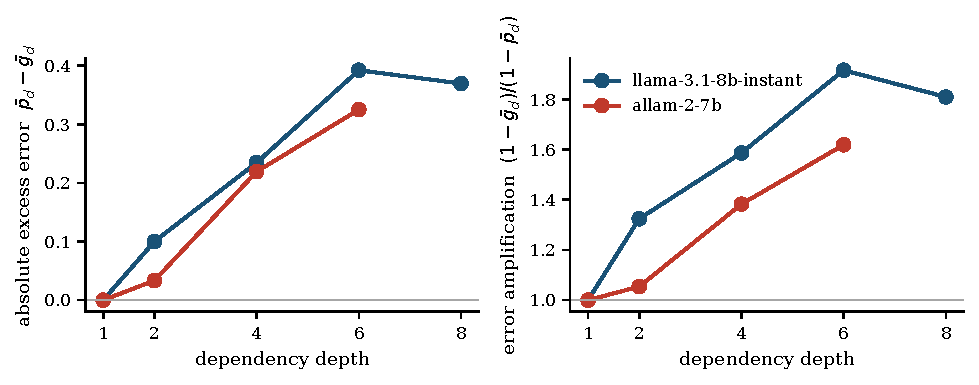
\includegraphics[width=0.92\textwidth]{fig_metric_sensitivity.pdf}
\caption{The propagation pattern is not specific to $L_d=1-\bar g_d/\bar p_d$. Absolute excess error grows to 0.392 and 0.325 by depth 6; free-running errors are amplified by factors of 1.916 and 1.619 relative to baseline errors. Both metrics plateau or terminate after depth 6 rather than supporting strict monotonicity.}
\label{fig:metric-sensitivity}
\end{figure}

\section{What each scoring regime identifies}
\label{app:scorers}

\begin{table}[h]
\centering
\caption{Scoring regimes answer complementary questions.}
\scriptsize
\begin{tabular}{@{}p{0.20\textwidth}p{0.20\textwidth}p{0.24\textwidth}p{0.25\textwidth}@{}}
\toprule
Scorer & Alternative paths & Primary estimand & Post-divergence limitation \\
\midrule
Canonical call/trajectory match & Usually no & Agreement with one reference & Local competence is confounded when the target has small $\epsilon_k$ \\
Conditional-on-state (ours) & Yes, one state at a time & Correct local continuation & Does not imply final task success \\
Milestone DAG (ToolSandbox) & Yes & Intermediate/final progress & Attribution depends on milestone coverage \\
Final-state tests (AppWorld, $\tau$-bench) & Yes & End-task state and side effects & Usually lacks per-call diagnosis \\
\bottomrule
\end{tabular}
\end{table}

\section{Posterior predictive check for the step-model fit}
\label{app:ppc}

Section~\ref{sec:central-result} states that the hierarchical fit is misspecified rather than
merely uncertain. This appendix shows the check behind that claim, and the reason a
conventional diagnostic does not detect it.

The fitted model implies that a call issued on a corrupted context succeeds with
probability $(1-\pi)p_k$, which is strictly positive for any $\pi<1$. Summed over the
corrupted-context calls in the suite, it therefore predicts a positive number of canonical
matches. The observed number is zero. We rebuilt the fitted model with one additional
observed node for that subset and drew from
\texttt{pm.sample\_posterior\_predictive} against the existing trace; no new model queries
were required.

\begin{table}[h]
\centering
\caption{Posterior predictive checks on two fits. The targeted check evaluates canonical
matches among corrupted-context calls only; the aggregate check evaluates total
free-running successes, which is the quantity such a fit is ordinarily judged on. Both
fits pass the aggregate check and fail the targeted one.}
\label{tab:ppc}
\scriptsize
\begin{tabular}{@{}lrr@{}}
\toprule
 & Real-model fit & Simulated-suite fit (control) \
\midrule
Corrupted-context calls & 869 & 9{,}624 \
Observed canonical matches & \textbf{0} & 1{,}648 \
Predicted mean & 67.7 & 3{,}173 \
Predicted 89\% interval & $[39,\ 98]$ & $[2{,}899,\ 3{,}427]$ \
Minimum over 6{,}000 replicates & 10 & 2{,}427 \
Targeted check, $\Pr(\text{rep}\le\text{obs})$ & $0.000$ & $0.000$ \
\midrule
Aggregate check, Bayesian $p$ & \textbf{0.420} & \textbf{0.282} \
\bottomrule
\end{tabular}
\end{table}

\begin{figure}[h]
\centering
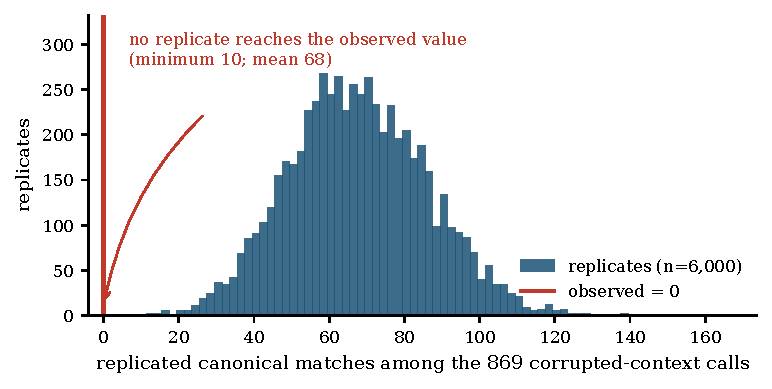
\includegraphics[width=0.82\textwidth]{fig_ppc.pdf}
\caption{Posterior predictive distribution of canonical matches among the 869
corrupted-context calls in the real-model fit, against the observed value. No replicate
reaches the observation; the smallest of 6{,}000 is 10.}
\label{fig:ppc}
\end{figure}

Two points follow. First, \textbf{the conventional check would have certified this fit as
adequate}. Replicated total free-running successes match the observation closely
($p=0.420$), because the marginal rate $g_k$ averages over clean and corrupted contexts and
the clean ones dominate the counts. A posterior predictive check aimed at the aggregate is
structurally blind to a failure confined to the corrupted subset, so passing it is not
evidence that the step model describes post-divergence behavior. Reporting an aggregate
predictive check alongside boundary-valued severity posteriors is therefore not a safeguard.

Second, the same targeted check fails on the simulated suite, where the generating policies
\emph{were} configured to recover and the observed count is a substantial 1{,}648. The fit
over-predicts there too, by roughly a factor of two. The over-prediction is thus a property
of the fit --- which under-estimates severity, so $(1-\pi)$ is too large --- and not an
artifact peculiar to real data sitting at a scorer-imposed boundary. This is what
distinguishes the finding from a claim that real models are simply harder to fit.


\end{document}